\documentclass[10pt]{beamer}
\mode<presentation>{
\usetheme{Madrid}
%\setbeamertemplate{caption}[numbered]
%\setbeamertemplate{footline} % To remove the footer line in all slides uncomment this line
\setbeamertemplate{footline}[page number] % To replace the footer line in all slides with a simple slide count uncomment this line
\setbeamertemplate{navigation symbols}{}
}

\usepackage{amsmath}
\usepackage{graphicx}
\usepackage{mathtools}
\usepackage[font={scriptsize}]{caption}

\title[Ruido en circuitos gen\'eticos]{Modelos de ruido en circuitos gen\'eticos}
\author{Luis Alberto Guti\'errez L\'opez}
\institute[Uniandes]{Universidad de los Andes\\
Departamento de F\'isica\\
\medskip
}
\date{Octubre 2 de 2015}

\begin{document}

\begin{frame}
\titlepage
\end{frame}

\begin{frame}
\frametitle{Expresi\'on gen\'etica}

\begin{figure}[p]
    \centering
    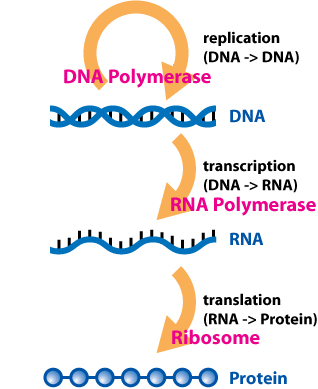
\includegraphics[width=0.3\textwidth]{dogma.jpg}\\
    \tiny Tomado de: \url{https://en.wikipedia.org/wiki/Central_dogma_of_molecular_biology}.
\end{figure}

\begin{figure}[p]
    \centering
    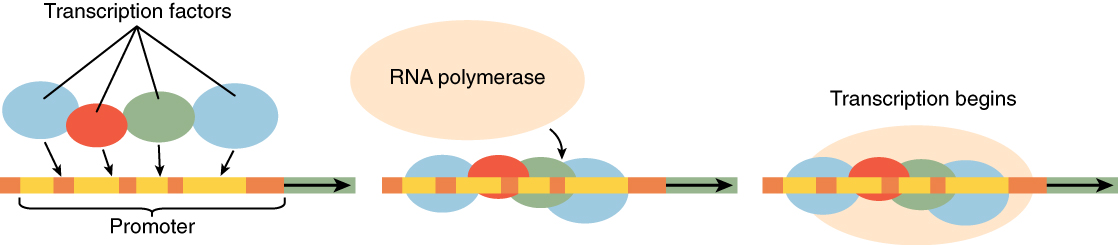
\includegraphics[width=0.8\textwidth]{tf1.jpg}\\
    \tiny Tomado de \url{http://oerpub.github.io/epubjs-demo-book/content/m46036.xhtml}.
\end{figure}
\end{frame}

\begin{frame}
\frametitle{Circuitos gen\'eticos}

\begin{figure}[p]
    \centering
    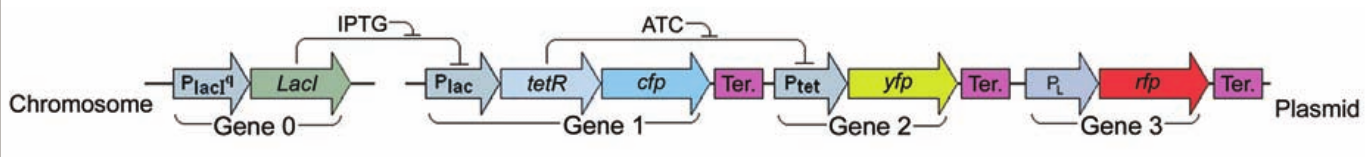
\includegraphics[width=0.9\textwidth]{circuitex.png}\\
    \tiny \cite{pedraza05}.
\end{figure}

\begin{figure}[p]
    \centering
    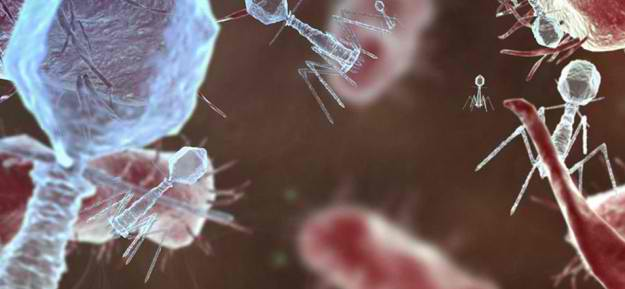
\includegraphics[width=0.2\textwidth]{phageim.jpg}\\
    \tiny Tomado de: \url{phages.org}.
\end{figure}

\begin{figure}[p]
    \centering
    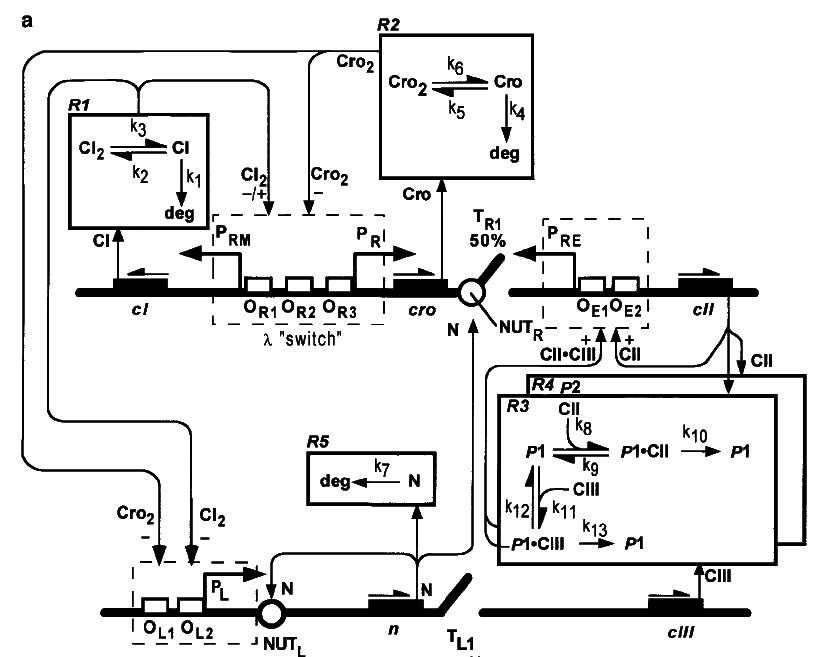
\includegraphics[width=0.35\textwidth]{lambdacirc.png}\\
    \tiny \cite{arkin98}.
\end{figure}

\end{frame}

\begin{frame}
\frametitle{Biolog\'ia de sistemas}
\begin{itemize}
\item Holismo (SysBio.) vs. reduccionismo (Bio.).
\item Interacciones entre partes  vs. estructura y funcionamiento de elementos individuales.
\item Ingenier\'ia (e.g. motifs).
\end{itemize}
\end{frame}

\begin{frame}
\frametitle{Ruido en circuitos gen\'eticos}
\begin{itemize}
\item Fluctuaciones aleatorias en expresi\'on gen\'etica.
\item En transcripci\'on y traducci\'on: Colisiones aleatorias entre mol\'eculas que se encuentran en bajo n\'umero (Intr\'inseco).
\item Otros factores como la divisi\'on celular y la variablidad del ambiente (Extr\'inseco).
\begin{align*}
\eta_X &= \frac{\sigma_X}{\langle X \rangle}.\\[1.5ex]
\nu_X &= \frac{\sigma^2_X}{\langle X \rangle}.
\end{align*}
\end{itemize}
\end{frame}


\begin{frame}
\frametitle{Manifestaciones del ruido}
\begin{figure}[p]
    \centering
    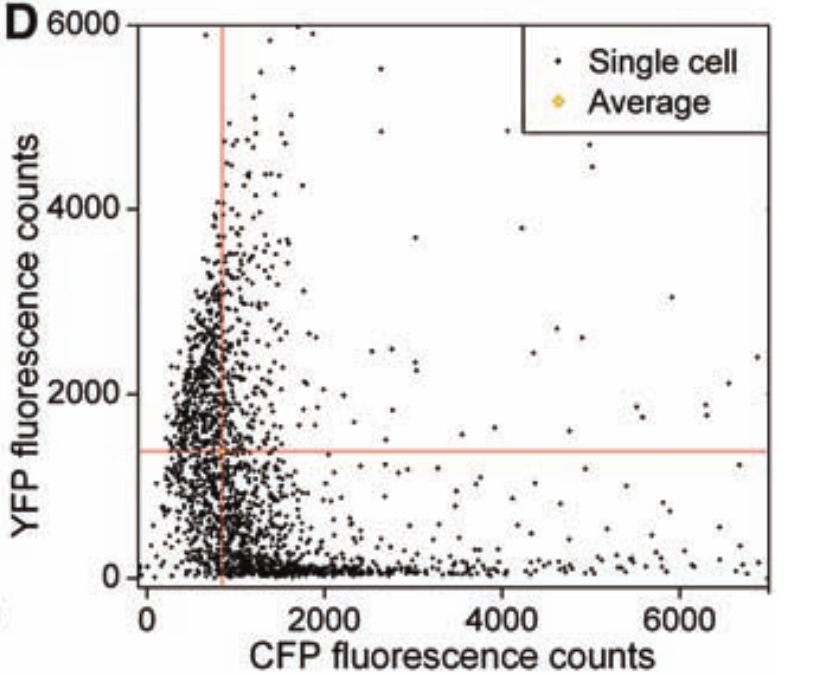
\includegraphics[width=0.5\textwidth]{noiseGFP.png}\\
    \tiny \cite{pedraza05}.
\end{figure}
\end{frame}


\begin{frame}
\frametitle{Estrategias ante el ruido}
\hspace{20 mm} \textbf{Robustez} \hspace{40 mm} \textbf{Variabilidad}
\begin{columns}[c]
\column{.5\textwidth}
\begin{figure}[p]
    \centering
    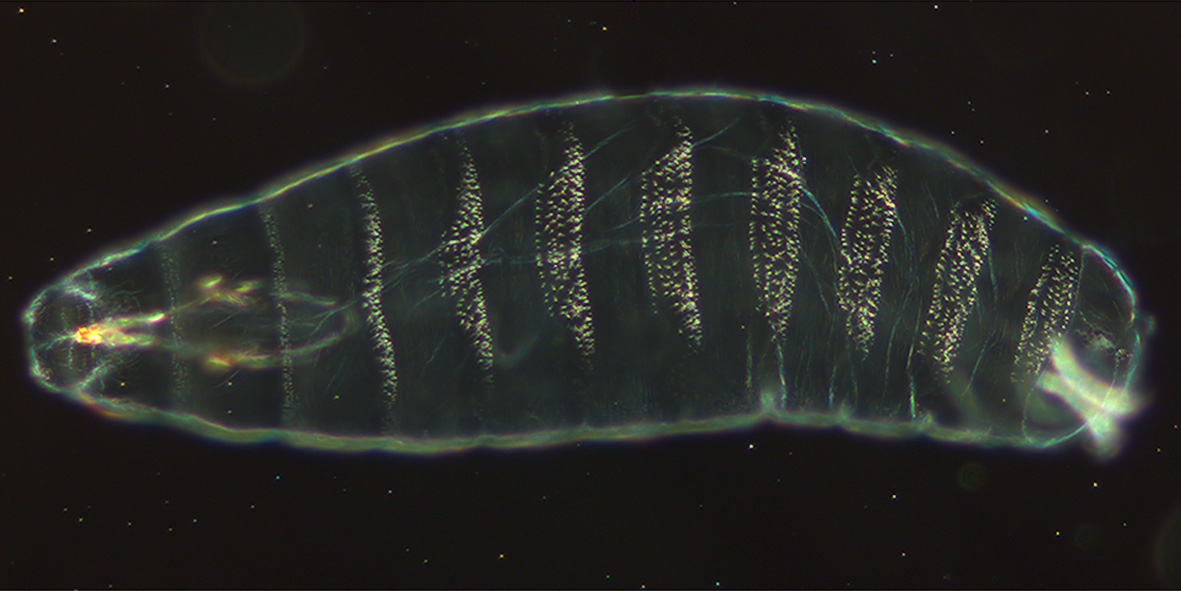
\includegraphics[width=0.9\textwidth]{drosophila.jpg}\\
    \tiny Tomado de: \url{https://en.wikipedia.org/wiki/Drosophila_embryogenesis}.
\end{figure}

\column{.5\textwidth}
\begin{figure}[p]
    \centering
    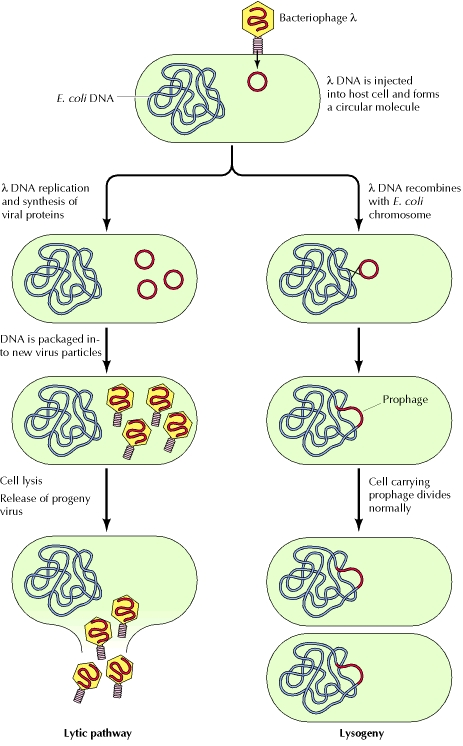
\includegraphics[width=0.7\textwidth]{lambda.jpg}\\
    \tiny \cite{cooper00}.
\end{figure}
\end{columns}
\end{frame}

\begin{frame}
\frametitle{Ruido intr\'inseco en circuitos gen\'eticos}
\begin{figure}[p]
    \centering
    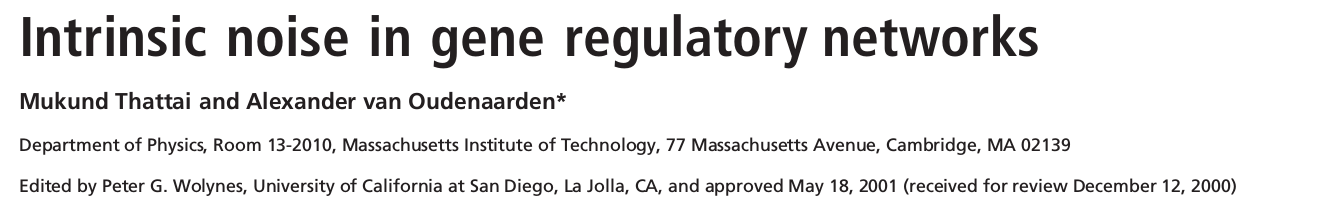
\includegraphics[width=1\textwidth]{title.png}\\
    \tiny \cite{thattai01}.
\end{figure}
\end{frame}

\begin{frame}
\frametitle{Suposiciones y ecuaciones deterministas}
\begin{columns}[c]
\column{0.5\textwidth}
\begin{itemize}
\item La tasa de producci\'on de ARN es cte. $k_R$. 
\item Tasa de producci\'on de prote\'inas cte. por cada ARN $k_P$.
\item Tasas de decaimiento $\gamma_R$ y $\gamma_P$.
\item $k_R \sim 1 \frac{\text{RNA}}{\text{min}}.$
\item $k_P \sim 60 \frac{\text{prote\'inas}}{\text{RNA min}}.$
\item $\gamma_R \sim \frac{1}{5\text{ min}}.$
\item $\gamma_R \sim \frac{1}{30\text{ min}}.$
\end{itemize}
\column{0.4\textwidth}
\begin{figure}[p]
    \centering
    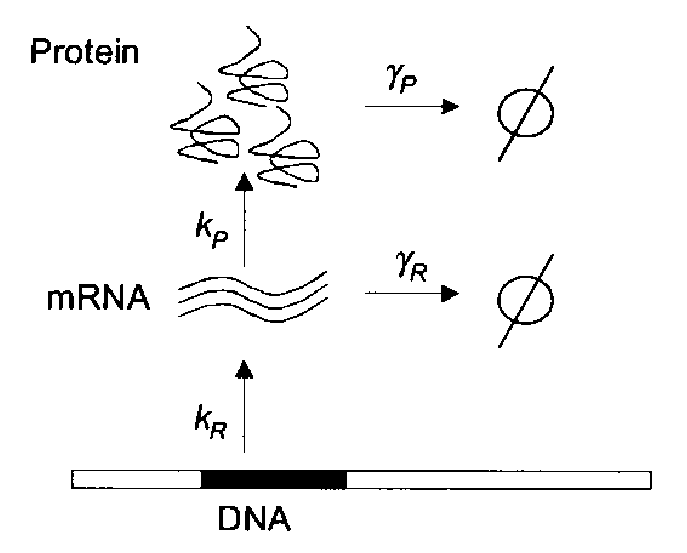
\includegraphics[width=1\textwidth]{expressionsimple.png}\\
    \tiny \cite{thattai01}.
\end{figure}
\begin{align*}
\dot{r}(t) &= k_R - \gamma_Rr(t).\\
\dot{p}(t) &= k_Pr(t) - \gamma_Pp(t).
\end{align*}
\end{columns}
\end{frame}

\begin{frame}
\frametitle{Generalizaci\'on de ecuaciones deterministas}

Las ecuaciones

\begin{align*}
\dot{r}(t) &= k_r - \gamma_rr(t),\\
\dot{p}(t) &= k_pr(t) - \gamma_pp(t),
\end{align*}

pueden ser escritas como

\begin{equation*}
\mathbf{\dot{q}} = (A - \Gamma)\mathbf{q}.
\end{equation*}

Donde $\mathbf{q}^T \coloneqq (d, r, p)$ y

\begin{align*}
A \coloneqq \bordermatrix{
  ~ & (d) & (r) & (p) \cr
  (d) & 0 & 0 & 0 \cr
  (r) & k_R & 0 & 0 \cr
  (p) & 0 & k_P & 0 \cr}, \quad \quad
\Gamma \coloneqq \bordermatrix{
  ~ & (d) & (r) & (p) \cr
  (d) & 0 & 0 & 0 \cr
  (r) & 0 & \gamma_R & 0 \cr
  (p) & 0 & 0 & \gamma_P \cr}.\\
\end{align*}
\end{frame}

\begin{frame}
\frametitle{Ecuaci\'on maestra}
\begin{figure}[p]
    \centering
    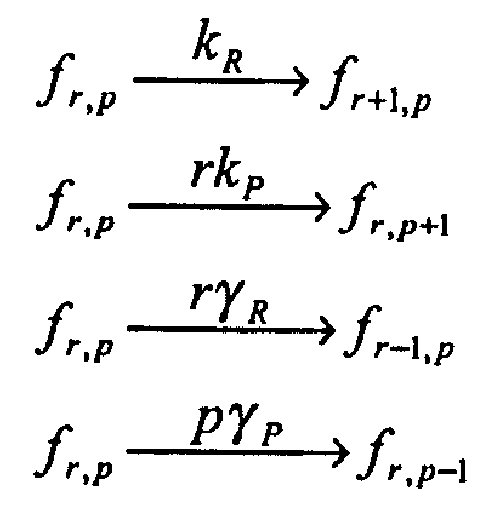
\includegraphics[width=0.3\textwidth]{scheme1.png}\\
    \tiny \cite{thattai01}.
\end{figure}
\begin{align*}
\frac{d{f}(r,p)}{dt} &= k_Rf(r-1,p) - k_Rf(r,p) + k_Prf(r,p-1) - k_Prf(r,p)\\
&+ \gamma_R(r+1)f(r+1,p) - \gamma_Rrf(r,p) + \gamma_P(p+1)f(r,p+1) - \gamma_Ppf(r,p).
\end{align*}
\end{frame}

\begin{frame}
Se puede realizar en general. Si $\mathbf{q}^T \coloneqq (q_1,q_2,\dots,q_i,\dots,q_n)$, 
\begin{figure}[p]
    \centering
    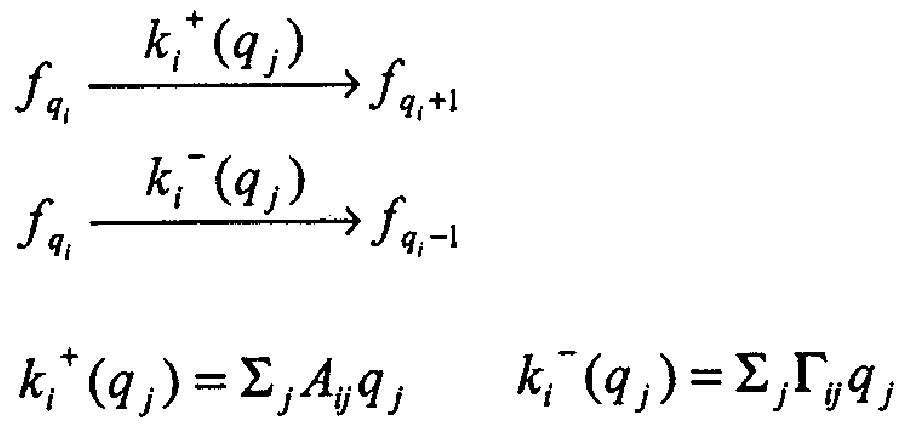
\includegraphics[width=0.6\textwidth]{scheme2.png}\\
    \tiny \cite{thattai01}.
\end{figure}
la ecuaci\'on maestra queda
\begin{align*}
\dot{f}(\mathbf{q}) &= \sum_{i=1}^n \: \sum_{j=1}^n \left[\, \left(A_{ij}q_j\right) \left(f(q_i-1) - f(q_i)\right) \, \right] \\
 & + \Gamma_{ii}(q_{i}+1)f(q_i+1) -\Gamma_{ii}q_if(q_i) \: .
\end{align*}
\end{frame}
%\dot{f}(q_i) = \sum_j \left[\left(A_{ij}q_j\right) \left(f(q_i-1) - f(q_i)\right)\right] + \Gamma_{ii}(q_{i}+1)f(q_i+1) -\Gamma_{ii}q_if(q_i)
%\dot{f}_{q_i} = \sum_j \left[\left(A_{ij}q_j\right) \left(f_{q_i-1} - f_{q_i}\right)\right] + \Gamma_{ii}(q_{i}+1)f_{q_i+1} -\Gamma_{ii}q_if_{q_i}

\begin{frame}
\frametitle{Funci\'on generadora de momentos}

$$F(z_1,\dots,z_n) \coloneqq \sum^{\infty}_{q_1,\dots,q_n = 0}z_1^{q_1} \dots z_n^{q_n}f(q_1,\dots,q_n).$$

Para todos $i, j = 1,\dots,n$  se cumple que: ($|_1 \coloneqq |_{z_1,\dots,z_n=1}$)

$$ \left. F\right|_1 = 1. $$
$$ \left. \frac{\partial F}{\partial z_i} \right|_1 = \langle q_i \rangle. $$
$$ \left. \frac{\partial^2 F}{\partial z_i \partial z_j} \right|_1 = \langle q_iq_j \rangle, \quad i\neq j.$$
$$ \left. \frac{\partial^2 F}{\partial z_i^2} \right|_1 = \langle q_i(q_i - 1) \rangle. $$
\end{frame}

\begin{frame}
La ec. para $F$ es

$$\dot{F} = \sum_{i=1}^n(1-z_i)\left(\Gamma_i\frac{\partial F}{\partial z_i} - \sum_{j=1}^n A_{ij}z_j\frac{\partial F}{\partial z_j} \right).$$

En s.s. y derivando respecto a $z_l$

\begin{align*}
0 =& \sum_{i=1}^n (1-z_i)\left(\Gamma_i\frac{\partial^2F}{\partial z_i \partial z_j} - \sum_{j=1}^nA_{ij}\left( z_j\frac{\partial^2F}{\partial z_j\partial z_l} + \delta_{lj}\frac{\partial F}{\partial z_j} \right) \right) \\
&-\delta_{il}\left(\Gamma_i \frac{\partial F}{\partial z_i} - \sum_{i=1}^nA_{ij}z_j\frac{\partial F}{\partial z_j} \right).
\end{align*}

Evaluando en 1

$$0 = -\Gamma_l \langle q_l \rangle + \sum_{j=1}^nA_{lj}\langle q_j \rangle. $$

\end{frame}
\begin{frame}

$$\sum_{j=1}^n\left( A_{lj} - \delta_{ij}\Gamma_{lj}\right) \langle q_j \rangle.$$

$$\left(\mathbf{A} - \mathbf{\Gamma}\right)\langle \mathbf{q} \rangle = 0.$$

Derivando y evaluando en 1

\begin{align*}
0 =& \left(\Gamma_{ii}\left. \frac{\partial^2F}{\partial z_i \partial z_j}\right|_1 - \sum_{j=1}^nA{ij}z_j\left.\frac{\partial^2 F}{\partial z_j\partial z_l} \right|_1 - A_{il}\left.\frac{\partial F}{\partial z_l}\right|_1\right)\\
&+ \left(\Gamma_{ll}\left. \frac{\partial^2F}{\partial z_l \partial z_i}\right|_1 - \sum_{j=1}^nA{lj}z_j\left.\frac{\partial^2 F}{\partial z_j\partial z_i} \right|_1 - A_{li}\left.\frac{\partial F}{\partial z_i}\right|_1\right).
\end{align*}

$$0 = \left( \left( \mathbf{\Gamma} - \mathbf{A}\right) \nabla\nabla^TF|_1 - A\Theta F|_1 \right) +  \left( \left( \mathbf{\Gamma} - \mathbf{A}\right) \nabla\nabla^TF|_1 - A\Theta F|_1\right)^T,$$ 
$$\Theta_{ij} \coloneqq \delta_{ij}\frac{\partial}{\partial z_i}.$$

\end{frame}

\begin{frame}
\frametitle{Un s\'olo gen - Resultados}
\begin{align*}
\dot{r}(t) &= k_r - \gamma_rr(t),\\
\dot{p}(t) &= k_pr(t) - \gamma_pp(t),
\end{align*}

\begin{columns}[c]
\column{.45\textwidth}
\centering \textbf{Promedio}
\begin{align*}
\langle r \rangle &= \frac{k_R}{\gamma_R}.\\[1.5ex]
\langle p \rangle &= \frac{k_Rb}{\gamma_P}.
\end{align*}
\column{.5\textwidth}
\centering \textbf{Ruido}
\begin{align*}
\nu_r &= \frac{\sigma_r^2}{\langle r \rangle} = 1.\\[1.5ex]
\nu_p &= \frac{\sigma_p^2}{\langle p \rangle} = \frac{b}{1+\eta} + 1 \approx b + 1.
\end{align*}
\end{columns}

\vspace{3 mm}

\begin{equation*}
b \coloneqq \frac{k_P}{\gamma_R}, \quad \eta \coloneqq \frac{\gamma_P}{\gamma_R}.
\end{equation*}

\end{frame}

\begin{frame}
\frametitle{Autorregulaci\'on - Modelo}
\begin{figure}[p]
    \centering
    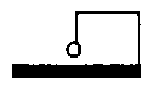
\includegraphics[width=0.2\textwidth]{autorreg.png}\\
    \tiny \cite{thattai01}.
\end{figure}
\begin{columns}[c]

\column{.5\textwidth}
\begin{figure}[p]
    \centering
    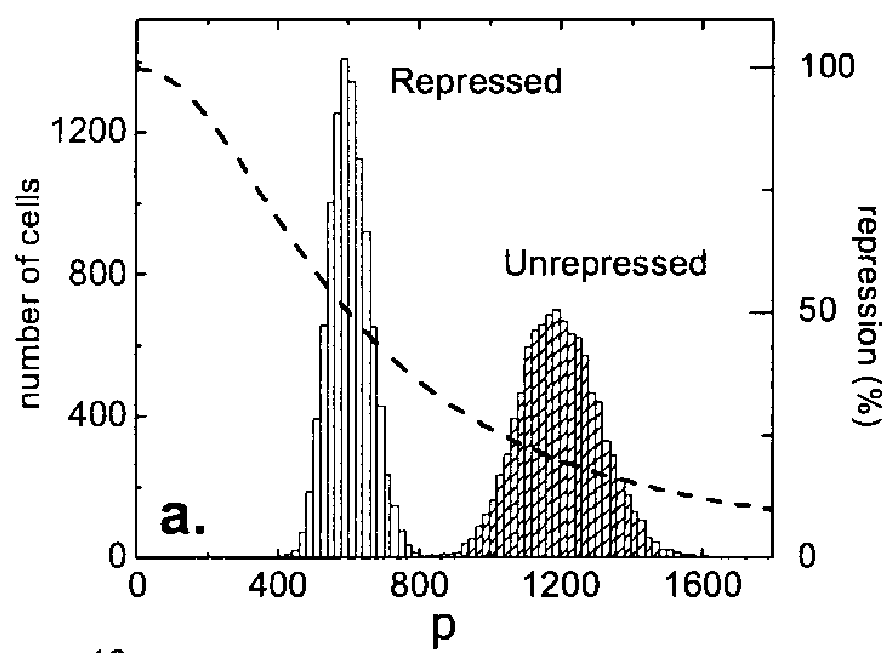
\includegraphics[width=1\textwidth]{graph3.png}\\
    \tiny \cite{thattai01}.
\end{figure}

\column{.5\textwidth}
\begin{itemize}
\item Ecuaci\'on de Hill.
\begin{equation*}
k_R = \frac{k_R^{\text{max}}}{1+(p/K_d)^n}.
\end{equation*}
\item Linearizar alrededor del promedio en estado estacionario.
\begin{equation*}
k_R \approx k_0-k_1p.
\end{equation*}
\begin{equation*}
A = 
\begin{pmatrix}
0 & 0 & 0 \\
k_0 & 0 & -k_1 \\
0 & k_P & 0
\end{pmatrix}.
\end{equation*}
\end{itemize}
\end{columns}
\end{frame}

\begin{frame}
\frametitle{Autorregulaci\'on - Resultados}
\begin{columns}[c]

\column{.45\textwidth}
\centering \textbf{Promedio}
\begin{align*}
%\langle r \rangle &= .\\[1.5ex]
\langle p \rangle &= \frac{1}{1+b\phi} \cdot \frac{k_0b}{\gamma_p}.
\end{align*}

\column{.5\textwidth}
\centering \textbf{Ruido}
\begin{align*}
%\nu_r &= .\\[1.5ex]
\nu_p &= \frac{1-\phi}{1+b\phi} \cdot \frac{b}{1+\eta}+1.
\end{align*}
\end{columns}

\vspace{3 mm}

\begin{equation*}
  b \coloneqq \frac{k_P}{\gamma_R}, \quad \eta \coloneqq \frac{\gamma_P}{\gamma_R}, \quad \phi \coloneqq \frac{k_1}{\gamma_P}.
\end{equation*}

\begin{figure}[p]
    \centering
    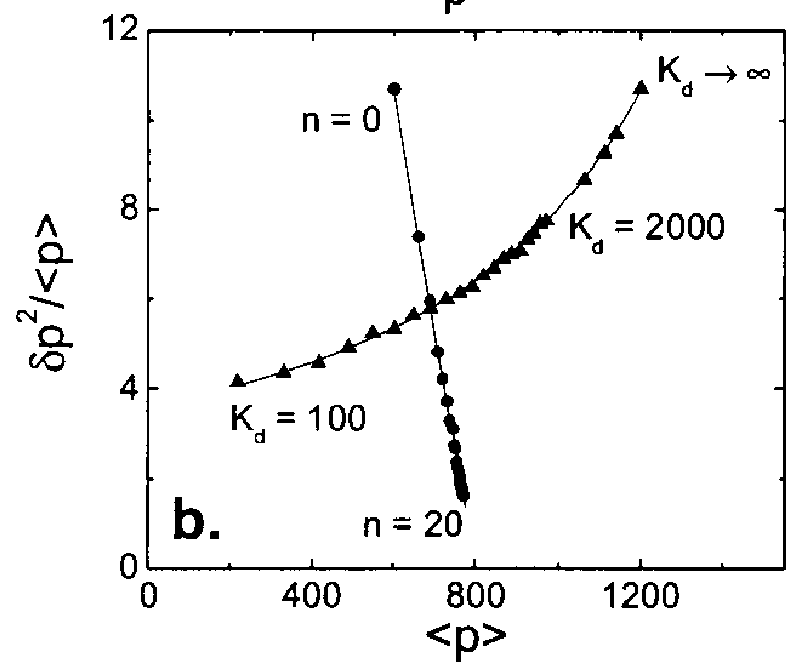
\includegraphics[width=0.5\textwidth]{graph5.png}\\
    \tiny \cite{thattai01}.
\end{figure}

\end{frame}


\begin{frame}
\frametitle{En general}
\begin{columns}[c]
\column{.6\textwidth}
\begin{figure}[p]
    \centering
    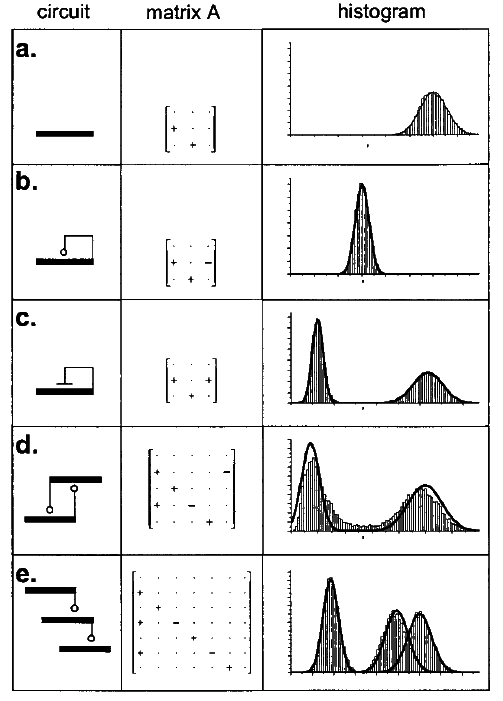
\includegraphics[width=0.75\textwidth]{graph4.png}\\
    \tiny \cite{thattai01}.
\end{figure}
\column{.4\textwidth}
\begin{itemize}
\item Posibilidad de biestabilidad.
\item Linearizar alrededor de cada punto de equilibrio.
\end{itemize}
\end{columns}
\end{frame}

\begin{frame}
\frametitle{Problemas}
\begin{itemize}
\item Hay muchas otras fuentes de ruido que no se consideran.
\item Modelo linearizado.
\item No sirve para explicar el comportamiento lejos de los puntos fijos si el sistema es no lineal.
\end{itemize}
\end{frame}

%AQUI CORTE

%\iffalse
\begin{frame}
\frametitle{Propagaci\'on del Ruido}
\begin{figure}[p]
    \centering
    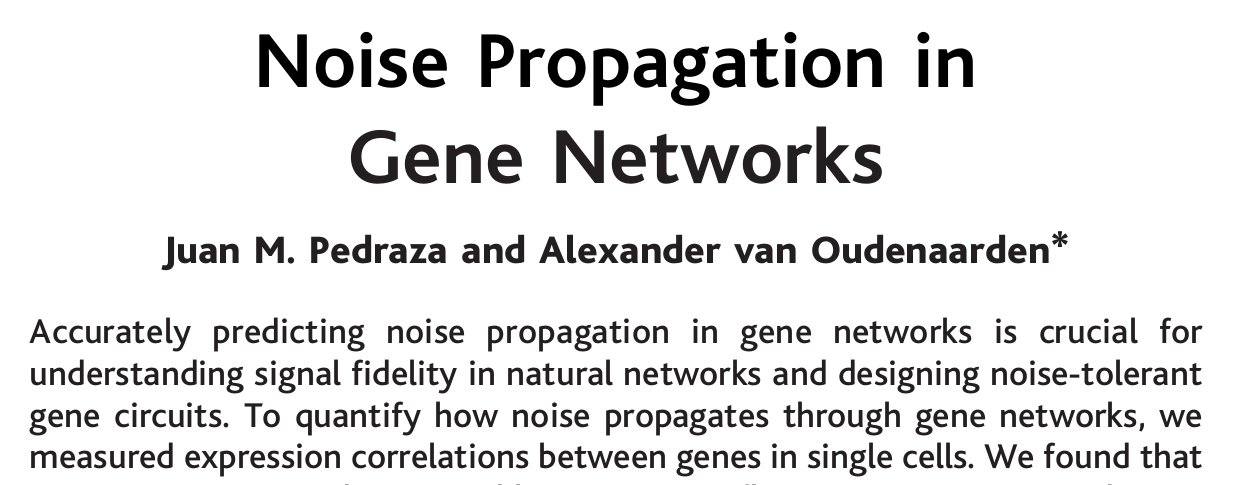
\includegraphics[width=0.8\textwidth]{pedtitle.png}\\
    \tiny \cite{pedraza05}.
\end{figure}

\begin{figure}[p]
    \centering
    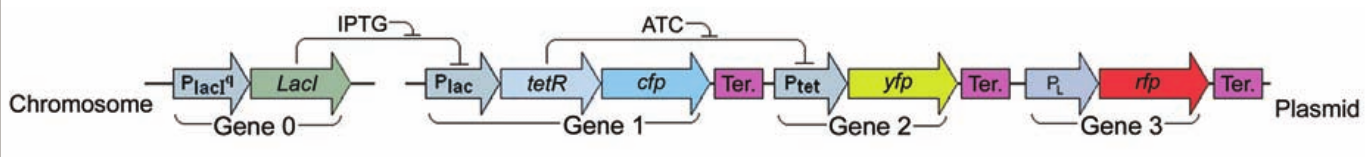
\includegraphics[width=0.9\textwidth]{circuitex.png}\\
    \tiny \cite{pedraza05}.
\end{figure}

\end{frame}

\begin{frame}
\frametitle{Ecuaci\'on de Langevin}

Para el gen $0$

\begin{equation*}
  \dot{p_0}(t) = k - \gamma p_0(t) + \mu_0(t) + \xi_{0G}(t).
\end{equation*}

\begin{align*}
  &\langle \mu_0 \rangle = \langle \xi_{0G} \rangle = 0,\\
  &\langle \mu_0(t)\mu_0(t+\tau) \rangle = 2 \gamma \tilde{b_0} \overline{p_0} \delta(\tau),\\
  &\langle \xi_{0G}(t)\xi_{0G}(t+\tau) \rangle = 2 \gamma \eta_G^2 \overline{p_0}^2 \delta(\tau).
\end{align*}

Escribiendo $\Delta p_0 \coloneqq p_0 - \bar{p_0}$,

\begin{align*}
   \dot{\Delta p_0} &= k - \gamma \Delta p_0 - \gamma \overline{p_0} + \mu _0 + \xi_{0G}\\
   & = -\gamma \Delta p_0 + \mu_0 + \xi_{0G}.
\end{align*}

\end{frame}
\begin{frame}
Aplicando transformada de Fourier

$$i\omega (\Delta p_0) = -\gamma (\Delta p_0) + \mu_0 + \xi_{0G}.$$

Despejando $\Delta p_0$, tomando norma al cuadrado y promediando

$$\langle \left| \Delta p_0 \right|^2 \rangle = \frac{\langle \left| \mu_0 \right|^2 \rangle + \langle \left| \xi_{0G} \right|^2 \rangle}{\omega^2+\gamma^2}.$$

Del teorema de Wiener-Khinchin

$$\langle \left| \Delta p_0 \right|^2 \rangle = \left( 2 \gamma \tilde{b_0} \overline{p_0} + 2 \gamma \eta_G^2 \overline{p_0}^2 \right) \frac{1}{\omega^2 + \gamma^2}$$

\end{frame}
\begin{frame}

Antitransformando

$$\langle \Delta p_0^2 \rangle = \sigma^2(p_0) = 2 \gamma \overline{p_0}\left(  \tilde{b_0} + \eta_G^2 \overline{p_0} \right) \frac{1}{2 \pi} \int ^{\infty}_{-\infty} \frac{d\omega}{\omega^2+\gamma^2}$$.

La integral es $2i\pi \frac{1}{2i\gamma}$. Entonces

$$\sigma^2(p_0) =  \overline{p_0} \left( \tilde{b_0} + \eta_G^2p_0 \right)$$.

Y el ruido es

$$\eta_0^2 = \frac{\tilde{b_0}}{\overline{p_0}} + \eta_G^2 = \eta_{0_{\text{int}}}^2 + \eta_G^2$$.

\end{frame}
%\fi

\begin{frame}
\frametitle{Referencias}
\footnotesize{
\begin{thebibliography}{99}

\bibitem[Arkin et al., 1998]{arkin98} Arkin, A., Ross, J. \& McAdams H. H. (1998).
\newblock Stochastic Kinetic Analysis of Developmental Pathway Bifurcation in Phage $\lambda$-Infected Escherichia coli Cells.
\newblock \emph{Genetics} 149, 1633 -- 1648.

\bibitem[Cooper, 2000]{cooper00} Cooper, G. M. (2000).
\newblock The Cell, A Molecular Approach. 2nd Edition.
\newblock Sunderland (MA): Sinauer Associates.

\bibitem[Thattai \& van Oudenaarden, 2001]{thattai01} Thattai, M. \& van Oudenaarden, A. (2001).
\newblock Intrinsic noise in gene regulatory networks.
\newblock \emph{PNAS} 98(15), 8614 -- 8619.

\bibitem[Pedraza \& van Oudenaarden, 2005]{pedraza05} Pedraza, J. M. \& van Oudenaarden, A. (2005).
\newblock Noise Propagation in Gene Networks.
\newblock \emph{Science} 307, 1965 -- 1969.

\bibitem[Kaern et al., 2005]{kaern05} Kaern, M., Elston, T. C., Blake, W. J. \& Collins, J. J. (2005).
\newblock Stochasticity in gene expression: from theories to phenothypes.
\newblock \emph{Nat Rev Genet} 6(6), 451 -- 464.

\end{thebibliography}
}
\end{frame}

\end{document}
